

\documentclass[11pt]{article}
\usepackage{acl2015}
\usepackage{times}
\usepackage{latexsym}
% \setlength\titlebox{5cm}    % Expanding the titlebox

%%% Custom additions %%%
% \usepackage{hyperref}
\usepackage{url}
\usepackage[leqno, fleqn]{amsmath}
\usepackage{amssymb}
\usepackage{qtree}
\usepackage{graphicx}
\usepackage{booktabs}
\usepackage{colortbl}
% \usepackage{caption}
\usepackage{subcaption}
\usepackage{color}
\usepackage{xcolor}
\usepackage{tikz}
\usepackage{ifthen}

\newcount\colveccount
\newcommand*\colvec[1]{
        \global\colveccount#1
        \begin{bmatrix}
        \colvecnext
}
\def\colvecnext#1{
        #1
        \global\advance\colveccount-1
        \ifnum\colveccount>0
                \\
                \expandafter\colvecnext
        \else
                \end{bmatrix}
        \fi
}


\newcommand{\nateq}{\equiv}
\newcommand{\natind}{\mathbin{\#}}
%\newcommand{\natneg}{\raisebox{2px}{\tiny\thinspace$\wedge$\thinspace}}
\newcommand{\natneg}{\mathbin{^{\wedge}}}
\newcommand{\natfor}{\sqsubset}
\newcommand{\natrev}{\sqsupset}
\newcommand{\natalt}{\mathbin{|}}
\newcommand{\natcov}{\mathbin{\smallsmile}}

\newcommand{\plneg}{\mathop{\textit{not}}}
\newcommand{\pland}{\mathbin{\textit{and}}}
\newcommand{\plor}{\mathbin{\textit{or}}}

% Strikeout
\newlength{\howlong}\newcommand{\strikeout}[1]{\settowidth{\howlong}{#1}#1\unitlength0.5ex%
\begin{picture}(0,0)\put(0,1){\line(-1,0){\howlong\divide\unitlength}}\end{picture}}

\newcommand{\True}{\texttt{T}}
\newcommand{\False}{\texttt{F}}
\usepackage{stmaryrd}
\newcommand{\sem}[1]{\ensuremath{\llbracket#1\rrbracket}}

\newcommand{\mynote}[1]{{\color{blue}#1}}

\newcommand{\tbchecked}[1]{{\color{red}#1}}

\usepackage{gb4e}
\noautomath

\def\ii#1{\textit{#1}}
\newcommand{\word}[1]{\emph{#1}}

%%%%%%%%%%%%%%%%%%%%%%%%%%%%%%%%%%%%%%%%%%%%%%%%%%%%%%%%%%%%%%%%%%%%%%
%%%%% Code to simulate natbib's citealt, which prints citations with
%%%%% no parentheses:

\makeatletter
\def\citealt{\def\citename##1{{\frenchspacing##1} }\@internalcitec}
\def\@citexc[#1]#2{\if@filesw\immediate\write\@auxout{\string\citation{#2}}\fi
  \def\@citea{}\@citealt{\@for\@citeb:=#2\do
    {\@citea\def\@citea{;\penalty\@m\ }\@ifundefined
       {b@\@citeb}{{\bf ?}\@warning
       {Citation `\@citeb' on page \thepage \space undefined}}%
{\csname b@\@citeb\endcsname}}}{#1}}
\def\@internalcitec{\@ifnextchar [{\@tempswatrue\@citexc}{\@tempswafalse\@citexc[]}}
\def\@citealt#1#2{{#1\if@tempswa, #2\fi}}
\makeatother

%%%%%%%%%%%%%%%%%%%%%%%%%%%%%%%%%%%%%%%%%%%%%%%%%%%%%%%%%%%%%%%%%%%%%%


%%% %%%

\title{As yet untitled paper chunk}

%\Thanks{}}

%\author{
%Samuel R.\ Bowman$^{\ast\dag}$ \\
%\texttt{sbowman@stanford.edu} \\[2ex]
%$^{\ast}$Stanford Linguistics \\
%\And
%Christopher Potts$^{\ast}$\\
%\texttt{cgpotts@stanford.edu} \\[2ex]
%$^{\dag}$Stanford NLP Group
%\And
%Christopher D.\ Manning$^{\ast\dag\ddag}$\\
%\texttt{manning@stanford.edu}\\[2ex]
%$^{\ddag}$Stanford Computer Science
%}

\author{First Author \\
  Affiliation / Address line 1 \\
  Affiliation / Address line 2 \\
  Affiliation / Address line 3 \\
  {\tt email@domain} \\\And
  Second Author \\
  Affiliation / Address line 1 \\
  Affiliation / Address line 2 \\
  Affiliation / Address line 3 \\
  {\tt email@domain} \\}

\date{}

\makeatletter
\newcommand{\@BIBLABEL}{\@emptybiblabel}
\newcommand{\@emptybiblabel}[1]{}
\definecolor{black}{rgb}{0,0,0}
\makeatother
\usepackage[breaklinks, draft, colorlinks, linkcolor=black, urlcolor=black, citecolor=black]{hyperref}

\begin{document}
\maketitle

% \begin{abstract}
Tree-structured neural networks aim to deliver a robust and principled method for representing sentence meaning, but these models largely have not outperformed simpler sequence-based models by substantial margins. We hypothesize that sequence models like LSTMs are able to discover and implicitly use the same kinds of recursive compositional structures that the tree-structured ones are built around---at least in cases where there are clear cues to that structure in the data---mitigating the advantage of the tree-structured models. We investigate this possibility by evaluating both models on an artificial task for which recursive compositional structure is crucial, and find that the sequence model is able to exploit the underlying structure, though it is less efficient at learning than the tree models, only succeeding after exposure to a larger and richer set of training data.
\end{abstract}

\section{Jointly learning parsing and semantic composition}

% TODO: Graph figure



\begin{figure}[tp]
  \centering\small
 	 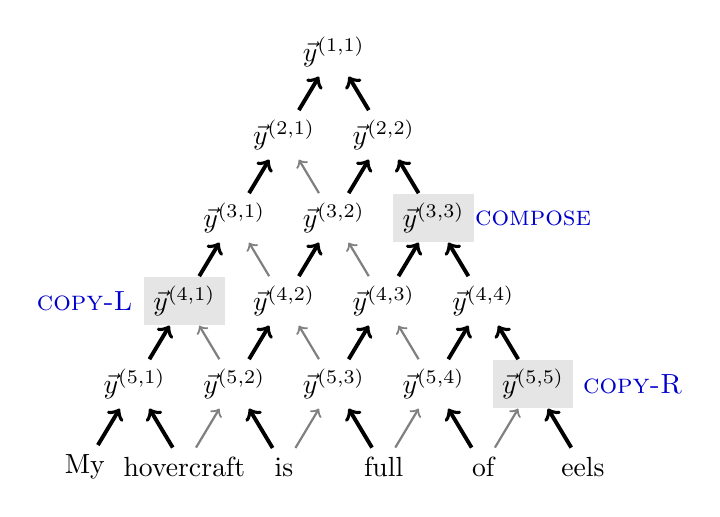
\begin{tikzpicture}
    \def\dx{18pt}
    \def\dy{30pt}
    \newcounter{i}
    \tikzstyle{highlight}=[fill=black!10]
    \tikzstyle{comment}=[color=blue!80!black]
    
    \stepcounter{i}\node  (\arabic{i}) at (0*\dx,6*\dy) {$\vec{y}^{(1, 1)}$};
    \stepcounter{i}\node  (\arabic{i}) at (-1*\dx,5*\dy) {$\vec{y}^{(2, 1)}$};
    \stepcounter{i}\node  (\arabic{i}) at (1*\dx,5*\dy) {$\vec{y}^{(2, 2)}$};
    \stepcounter{i}\node  (\arabic{i}) at (-2*\dx,4*\dy) {$\vec{y}^{(3, 1)}$};
    \stepcounter{i}\node  (\arabic{i}) at (0*\dx,4*\dy) {$\vec{y}^{(3, 2)}$};
    \stepcounter{i}\node[highlight]  (\arabic{i}) at (2*\dx,4*\dy) {$\vec{y}^{(3, 3)}$};
    \stepcounter{i}\node[highlight]  (\arabic{i}) at (-3*\dx,3*\dy) {$\vec{y}^{(4, 1)}$};
    \stepcounter{i}\node  (\arabic{i}) at (-1*\dx,3*\dy) {$\vec{y}^{(4, 2)}$};
    \stepcounter{i}\node  (\arabic{i}) at (1*\dx,3*\dy) {$\vec{y}^{(4, 3)}$};
    \stepcounter{i}\node  (\arabic{i}) at (3*\dx,3*\dy) {$\vec{y}^{(4, 4)}$};
    \stepcounter{i}\node  (\arabic{i}) at (-4*\dx,2*\dy) {$\vec{y}^{(5, 1)}$};
    \stepcounter{i}\node  (\arabic{i}) at (-2*\dx,2*\dy) {$\vec{y}^{(5, 2)}$};
    \stepcounter{i}\node  (\arabic{i}) at (0*\dx,2*\dy) {$\vec{y}^{(5, 3)}$};
    \stepcounter{i}\node  (\arabic{i}) at (2*\dx,2*\dy) {$\vec{y}^{(5, 4)}$};
    \stepcounter{i}\node[highlight]  (\arabic{i}) at (4*\dx,2*\dy) {$\vec{y}^{(5, 5)}$};
    \stepcounter{i}\node  (\arabic{i}) at (-5*\dx,1*\dy) {My};
    \stepcounter{i}\node  (\arabic{i}) at (-3*\dx,1*\dy) {hovercraft};
    \stepcounter{i}\node  (\arabic{i}) at (-1*\dx,1*\dy) {is};
    \stepcounter{i}\node  (\arabic{i}) at (1*\dx,1*\dy) {full};
    \stepcounter{i}\node  (\arabic{i}) at (3*\dx,1*\dy) {of};
    \stepcounter{i}\node  (\arabic{i}) at (5*\dx,1*\dy) {eels};
   
    \stepcounter{i}\node[comment]  (\arabic{i}) at (4*\dx,4*\dy) {\textsc{compose}};
    \stepcounter{i}\node[comment]  (\arabic{i}) at (-5*\dx,3*\dy) {\textsc{copy-L}};
    \stepcounter{i}\node[comment]  (\arabic{i}) at (6*\dx,2*\dy) {\textsc{copy-R}};
   
    \tikzstyle{extra} = [->, draw=black!50, line width=0.8pt]
    \tikzstyle{valid} = [->, draw=black, line width=1.4pt]

          \draw [valid] (2) -- (1);
          \draw [valid] (3) -- (1);
          
          \draw [valid] (4) -- (2);
          \draw [extra] (5) -- (2);
          \draw [valid] (5) -- (3);
          \draw [valid] (6) -- (3);
          
          \draw [valid] (7) -- (4);
          \draw [extra] (8) -- (4);
          \draw [valid] (8) -- (5);
          \draw [extra] (9) -- (5);
          \draw [valid] (9) -- (6);
          \draw [valid] (10) -- (6);
          
          \draw [valid] (11) -- (7);
          \draw [extra] (12) -- (7);
          \draw [valid] (12) -- (8);
          \draw [extra] (13) -- (8);
          \draw [valid] (13) -- (9);
          \draw [extra] (14) -- (9);
          \draw [valid] (14) -- (10);
          \draw [valid] (15) -- (10);
          
          \draw [valid] (16) -- (11);
          \draw [valid] (17) -- (11);
          \draw [extra] (17) -- (12);
          \draw [valid] (18) -- (12);
          \draw [extra] (18) -- (13);
          \draw [valid] (19) -- (13);
          \draw [extra] (19) -- (14);
          \draw [valid] (20) -- (14);
          \draw [extra] (20) -- (15);
          \draw [valid] (21) -- (15);
  \end{tikzpicture}

        \caption{The model structure used to compare \ii{turtle} and
          \ii{animal}.  Learned term representations are fed through
          either an NN or NTN comparison layer and then to a softmax
        classifier over the seven relations in Table~\ref{b-table}.}
  \label{sample-figure2}
\end{figure}

To compute the vector representation for a sentence, we populate the bottom row of the structure $\vec{y}^{(N,1...N)}$ with the embedddings of each of the words. We then compute the representations of each row starting at the second row from the bottom ($N - 1$), and moving from left to right. Computing one feature vector requires two steps. In the first step, a classifier produces a distribution $\vec{o}$ over the operations \{\textsc{copy-left, copy-right, compose}\}, and in the second step, that distribution is used to compute a feature vector $\vec{y}$.

To compute the distribution over operations at one node, $\vec{o}^{(i, j)}$, 




Choose an operation

row i
col j
amount of context C

To compute the vector representation for a sentence

\begin{equation} 
\label{TreeRNN}
\vec{o}^{(i,j)} = \text{softmax}(\mathbf{M_o} \colvec{7}
	{\vec{y}^{(i + 1, j - C + 1)}}
	{...}
	{\vec{y}^{(i + 1, j)}}
	{\vec{y}^{(i + 1, j + 1)}}
	{...}
	{\vec{y}^{(i + 1, j + C)}}
	{\vec{o}^{(i, j - 1)}}
	 + \vec{b}_o\,) \\
\end{equation}
	 
	 
\begin{equation}
\vec{y}^{(i,j)} = 
o^{(i, j)}_{1} \circ \vec{y^{(i + 1, j)}} +\\
o^{(i, j)}_{2} \circ \vec{y^{(i + 1, j + 1)}} +\\
o^{(i, j)}_{3} \circ \tanh(\mathbf{M_y} \colvec{2}{\vec{y}^{(i + 1, j)}}{\vec{y}^{(i + 1, j + 1)}} + \vec{b}_y)
\end{equation} 

For true relation $\rho$, and true operations $\omega^{(i,j)}$ for one example

\begin{equation}
loss = \lambda\theta^2-\ln(r_\rho) - \frac{1}{(N - 1)^2} \sum_{i = 1}^{N - 1} \sum_{j = 1}^{N - 1} \ln(o_{\omega^{(i,j)}})
\end{equation} 



\subsubsection*{Acknowledgments}

%%%

% \section*{Acknowledgments}

% Do not number the acknowledgment section.

\bibliographystyle{acl}
\bibliography{MLSemantics} 

\end{document}
